\documentclass[aspectratio=169,12pt]{beamer}
\usepackage[utf8]{inputenc}
\usepackage{amsmath, amssymb}
\usepackage{booktabs}
\usepackage{colortbl}
\usepackage{hyperref}
\usepackage{makecell}
\usepackage{ragged2e}
\usepackage{tikz}
\usetikzlibrary{arrows.meta, positioning, shapes.geometric, calc, tikzmark, shapes.misc, fit, decorations.pathreplacing, matrix}
\usepackage{tcolorbox}
\usepackage{array}
\usepackage{listings}
\usepackage{pgfkeys}
\usepackage[normalem]{ulem} 
\usetheme{Madrid}

% Custom colors - consolidated
\definecolor{correctgreen}{RGB}{0,150,0}
\definecolor{incorrectred}{RGB}{200,0,0}
\definecolor{counterblue}{RGB}{70,130,255}
\definecolor{highlightyellow}{RGB}{255,230,100}
\definecolor{lightblue}{RGB}{200,230,250}
\definecolor{darkblue}{RGB}{0,100,200}
\definecolor{highlightorange}{RGB}{255,200,100}

% PGF Keys for pipeline diagram configuration
\pgfkeys{
    /pipeline/.cd,
    % Stage colors
    ifcolor/.initial=lightblue,
    idcolor/.initial=lightblue,
    excolor/.initial=lightblue,
    memcolor/.initial=lightblue,
    wbcolor/.initial=lightblue,
    % Execution unit contents
    integercontent/.initial={},
    multiplycontent/.initial={},
    dividercontent/.initial={},
    % Instruction list
    instructions/.initial={},
    % Highlight colors for specific units
    highlightinteger/.initial=white,
    highlightmultiply/.initial=white,
    highlightdivider/.initial=white
}

% Macro for drawing the pipeline diagram
\newcommand{\drawPipeline}[1][]{%
    \pgfkeys{/pipeline/.cd,#1}%
    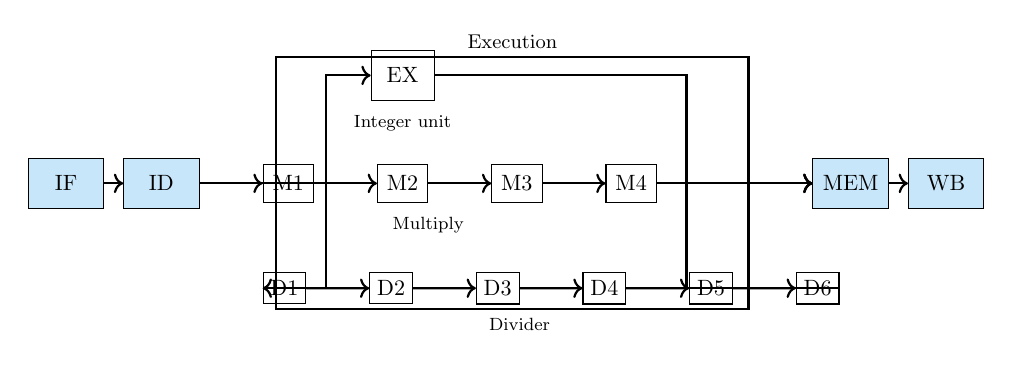
\begin{tikzpicture}[scale=0.8, transform shape]
        % Pipeline stages
        \node[draw, fill=\pgfkeysvalueof{/pipeline/ifcolor}, minimum width=1.2cm, minimum height=0.8cm] (IF) {IF};
        \node[draw, fill=\pgfkeysvalueof{/pipeline/idcolor}, minimum width=1.2cm, minimum height=0.8cm, right=0.3cm of IF] (ID) {ID};
        
        % Multiply pipeline (4 stages)
        \node[draw, fill=\pgfkeysvalueof{/pipeline/highlightmultiply}, minimum width=0.8cm, minimum height=0.6cm, right=of ID] (M1) {M1};
        \node[draw, fill=white, minimum width=0.8cm, minimum height=0.6cm, right=of M1] (M2) {M2};
        \node[draw, fill=white, minimum width=0.8cm, minimum height=0.6cm, right=of M2] (M3) {M3};
        \node[draw, fill=white, minimum width=0.8cm, minimum height=0.6cm, right=of M3] (M4) {M4};

        
        % Divider pipeline (multi-stage)
        \node[draw, fill=\pgfkeysvalueof{/pipeline/highlightdivider}, minimum width=0.6cm, minimum height=0.5cm, below right=of ID] (D1) {D1};
        \node[draw, fill=white, minimum width=0.6cm, minimum height=0.5cm, right=of D1] (D2) {D2};
        \node[draw, fill=white, minimum width=0.6cm, minimum height=0.5cm, right=of D2] (D3) {D3};
        \node[draw, fill=white, minimum width=0.6cm, minimum height=0.5cm, right=of D3] (D4) {D4};
        \node[draw, fill=white, minimum width=0.6cm, minimum height=0.5cm, right=of D4] (D5) {D5};
        \node[draw, fill=white, minimum width=0.6cm, minimum height=0.5cm, right=of D5] (D6) {D6};

        % Integer unit (single stage)
        \node[draw, fill=\pgfkeysvalueof{/pipeline/highlightinteger}, minimum width=1cm, minimum height=0.8cm, above=of M2] (EX) {EX};
         
        % Execution box (drawn after units to be in background)
        \node[draw, thick, minimum width=7.5cm, minimum height=4cm, right=1.2cm of ID] (execbox) {};
        \node[above=0 of execbox.north, anchor=south, font=\small] {Execution};
        
        % Labels for units
        \node[below=0.1cm of EX, font=\footnotesize] {Integer unit};
        \node[below=0.1cm of M2.south east, font=\footnotesize] {Multiply};
        \node[below=0.1cm of D3.south east, font=\footnotesize] {Divider};
        
        % MEM and WB stages
        \node[draw, fill=\pgfkeysvalueof{/pipeline/memcolor}, minimum width=1.2cm, minimum height=0.8cm, right=1cm of execbox] (MEM) {MEM};
        \node[draw, fill=\pgfkeysvalueof{/pipeline/wbcolor}, minimum width=1.2cm, minimum height=0.8cm, right=0.3cm of MEM] (WB) {WB};
        
        % Connections from IF to ID
        \draw[->, thick] (IF) -- (ID);
        
        % Connections from ID to execution units
        \draw[->, thick] (ID.east) -- ([xshift=2cm]ID.east) |- (EX.west);
        \draw[->, thick] (ID.east) -- (M1.west);
        \draw[->, thick] (ID.east) -- ([xshift=2cm]ID.east) |- (D1.west);
        
        % Connections within multiply pipeline
        \draw[->, thick] (M1) -- (M2);
        \draw[->, thick] (M2) -- (M3);
        \draw[->, thick] (M3) -- (M4);
        
        % Connections within divider pipeline
        \draw[->, thick] (D1) -- (D2);
        \draw[->, thick] (D2) -- (D3);
        \draw[->, thick] (D3) -- (D4);
        \draw[->, thick] (D4) -- (D5);
        \draw[->, thick] (D5) -- (D6);
        
        % Connections from execution units to MEM
        \draw[->, thick] (EX.east) -| ([xshift=-2cm]MEM.west) -- (MEM.west);
        \draw[->, thick] (M4.east) -- (MEM.west);
        \draw[->, thick] (D6.east) -| ([xshift=-2cm]MEM.west) -- (MEM.west);
        
        % Connection from MEM to WB
        \draw[->, thick] (MEM) -- (WB);
        
        % Add content to execution units if specified
        \pgfkeysgetvalue{/pipeline/integercontent}{\intcontent}
        \ifx\intcontent\empty\else
            \node[above=0.1cm of EX, font=\footnotesize, text=blue] {\intcontent};
        \fi
        
        \pgfkeysgetvalue{/pipeline/multiplycontent}{\mulcontent}
        \ifx\mulcontent\empty\else
            \node[above=0.1cm of M2, font=\footnotesize, text=blue] {\mulcontent};
        \fi
        
        \pgfkeysgetvalue{/pipeline/dividercontent}{\divcontent}
        \ifx\divcontent\empty\else
            \node[above=0.1cm of D3, font=\footnotesize, text=blue] {\divcontent};
        \fi
        
        % Instruction list
        \pgfkeysgetvalue{/pipeline/instructions}{\instlist}
        \ifx\instlist\empty\else
            \node[right=0.5cm of WB, align=left, font=\footnotesize] {\instlist};
        \fi
    \end{tikzpicture}%
}

% Macro for ROB diagram
\newcommand{\drawROB}[1]{%
    \begin{tikzpicture}[scale=0.8]
        \matrix (rob) [matrix of nodes, 
            nodes={draw, minimum width=2cm, minimum height=0.5cm, anchor=center},
            row sep=-\pgflinewidth,
            column sep=-\pgflinewidth,
            ] {
            #1
        };
        \node[left=0.3cm of rob-1-1] {P0};
        \node[left=0.3cm of rob-2-1] {P1};
        \node[left=0.3cm of rob-3-1] {P2};
        \node[left=0.3cm of rob-4-1] {P3};
        \node[below=0.1cm of rob-4-1] {$\vdots$};
        \node[left=0.3cm of rob-5-1] {Pn};
    \end{tikzpicture}
}

\title{Out-of-Order Execution\\(Part 1)}
\author{Computer Architecture}
\date{\today}

\begin{document}

\frame{\titlepage}

\begin{frame}{Execution of Instructions with Variable Execution Time}
    \begin{itemize}
        \item \textbf{Problem:} Single cycle Execution phase $\rightarrow$ The longest operation possible in the machine fixes the frequency
        \begin{itemize}
            \item Example: \textcolor{blue}{ADD/SUB=2ns, MUL=10ns, DIV=20ns} $\rightarrow$ \textcolor{red}{cc=20ns}
        \end{itemize}
        
        \item \textbf{Solution:} Implement a \textcolor{blue}{pipeline} in EXE
        \begin{itemize}
            \item Execution time of certain instructions is now variable (i.e. load with or without cache miss)
            \item More pipe stages = bigger penalty on misprediction and more data hazards (but generally an increase in CPI)
        \end{itemize}
    \end{itemize}
    
    \vspace{0.5cm}
    \centering
    \drawPipeline
\end{frame}

\begin{frame}{Example - In-Order Execution}
    \centering
    \drawPipeline[
        instructions={R1 $\leftarrow$ R1+4\\R2 $\leftarrow$ R3*R3\\R4 $\leftarrow$ R3+R4}
    ]
\end{frame}

\begin{frame}{Example - In-Order Step 1}
    \centering
    \drawPipeline[
        integercontent={R1 $\leftarrow$ R1+4},
        multiplycontent={R2 $\leftarrow$ R3*R3},
        instructions={R1 $\leftarrow$ R1+4\\R2 $\leftarrow$ R3*R3\\R4 $\leftarrow$ R3+R4},
        highlightinteger=highlightyellow,
        highlightmultiply=highlightyellow
    ]
\end{frame}

\begin{frame}{Example - In-Order Step 2}
    \centering
    \drawPipeline[
        integercontent={R4 $\leftarrow$ R3+R4},
        multiplycontent={R2 $\leftarrow$ R3*R3},
        instructions={R1 $\leftarrow$ R1+4\\R2 $\leftarrow$ R3*R3\\R4 $\leftarrow$ R3+R4},
        highlightinteger=highlightyellow,
        highlightmultiply=highlightyellow
    ]
    \vspace{0.5cm}
    
    \textcolor{red}{Note: R4 instruction is blocked waiting for R2 multiplication to complete!}
\end{frame}

\begin{frame}{Example - In-Order Multiple Steps}
    \centering
    \drawPipeline[
        multiplycontent={R2 $\leftarrow$ R3*R3},
        instructions={R1 $\leftarrow$ R1+4\\R2 $\leftarrow$ R3*R3\\R4 $\leftarrow$ R3+R4},
        highlightmultiply=highlightyellow
    ]
    \vspace{0.5cm}
    
    The multiplication continues through M2, M3, M4 stages...
\end{frame}

\begin{frame}{Example - In-Order Final Step}
    \centering
    \drawPipeline[
        integercontent={R4 $\leftarrow$ R3+R4},
        instructions={R1 $\leftarrow$ R1+4\\R2 $\leftarrow$ R3*R3\\R4 $\leftarrow$ R3+R4},
        highlightinteger=highlightyellow
    ]
    \vspace{0.5cm}
    
    Finally, R4 can execute after R2 completes
\end{frame}

\begin{frame}{Execution with Variable Time - The Problem}
    \begin{block}{Problem}
        A short operation might get "stuck" waiting for another operation of a different type to leave the Execution phase.
    \end{block}
    
    \begin{block}{Solution}
        Allow instructions of different types/pipelines to be executed \textbf{Out of Order}.
        \begin{itemize}
            \item Execute many independent instructions in parallel (in different pipelines)
            \item Improves CPI
            \item Execution must keep correctness of the code
        \end{itemize}
    \end{block}
    
    \begin{alertblock}{Note}
        If an operation gets "stuck" waiting for another operation of the same type to leave the Execution phase $\rightarrow$ \textbf{Structural Hazard} (need to add more execution units to solve).
    \end{alertblock}
\end{frame}

\begin{frame}{Example - Out-of-Order Execution}
    \centering
    \drawPipeline[
        integercontent={R1 $\leftarrow$ R1+4},
        multiplycontent={R2 $\leftarrow$ R3*R3},
        instructions={R1 $\leftarrow$ R1+4\\R2 $\leftarrow$ R3*R3\\R4 $\leftarrow$ R3+R4},
        highlightinteger=highlightyellow,
        highlightmultiply=highlightyellow
    ]
\end{frame}

\begin{frame}{Example - OOO Step 2}
    \centering
    \drawPipeline[
        integercontent={R4 $\leftarrow$ R3+R4},
        multiplycontent={R2 $\leftarrow$ R3*R3},
        instructions={R1 $\leftarrow$ R1+4\\R2 $\leftarrow$ R3*R3\\R4 $\leftarrow$ R3+R4},
        highlightinteger=correctgreen,
        highlightmultiply=highlightyellow
    ]
    \vspace{0.5cm}
    
    \textcolor{correctgreen}{R4 can execute immediately - no need to wait!}
\end{frame}

\begin{frame}{CPI Limitations}
    \begin{itemize}
        \item In \textbf{in-order} machines as we've known until today, the minimum CPI achievable is 1
        \item Even with OOO execution, this limit exists as long as we only allow parallel execution in the EXE stage
        \item If we allow multiple instructions to execute in parallel in \textbf{all stages}, we can break this barrier
    \end{itemize}
    
    \vspace{0.5cm}
    \centering
    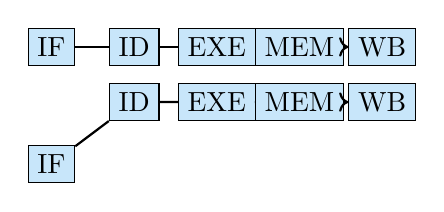
\begin{tikzpicture}[scale=0.7]
        \node[draw, fill=lightblue] (if1) at (0,0) {IF};
        \node[draw, fill=lightblue] (id1) at (1.5,0) {ID};
        \node[draw, fill=lightblue] (exe1) at (3,0) {EXE};
        \node[draw, fill=lightblue] (mem1) at (4.5,0) {MEM};
        \node[draw, fill=lightblue] (wb1) at (6,0) {WB};
        
        \node[draw, fill=lightblue, below=of if1] (if2) {IF};
        \node[draw, fill=lightblue] (id2) at (1.5,-1) {ID};
        \node[draw, fill=lightblue] (exe2) at (3,-1) {EXE};
        \node[draw, fill=lightblue] (mem2) at (4.5,-1) {MEM};
        \node[draw, fill=lightblue] (wb2) at (6,-1) {WB};
        
        \draw[->, thick] (if1) -- (id1) -- (exe1) -- (mem1) -- (wb1);
        \draw[->, thick] (if2) -- (id2) -- (exe2) -- (mem2) -- (wb2);
    \end{tikzpicture}
\end{frame}

\begin{frame}{Data Hazards}
    \begin{block}{RAW (Read After Write) - True Dependency}
        {\ttfamily\footnotesize
        (1) ADD R1, R2, R3\\
        (2) ADD R5, R6, R1  // Depends on R1 from previous instruction
        }
        The destination of the first instruction is a source in the second. This is a \textbf{true dependency} that must be maintained for program correctness.
    \end{block}
\end{frame}

\begin{frame}{New Data Hazards in OOO Execution}
    \begin{block}{WAR (Write After Read) - False Dependency}
        {\ttfamily\footnotesize
        (1) DIV R1, R2, R3  // Many cycles\\
        (2) ADD R5, R6, R1  // Depends on previous instruction\\
        (3) ADD R6, R7, R8  // WAR issue - might execute before (2)
        }
        \begin{itemize}
            \item The long division delays instruction (2)
            \item With OOO, instruction (3) (independent) executes before (2)
            \item Instruction (2) might read the new R6 value instead of the old one
        \end{itemize}
    \end{block}
\end{frame}

\begin{frame}{WAW (Write After Write) - False Dependency}
    \begin{block}{Example}
        {\ttfamily\footnotesize
        (1) DIV R1, R2, R3  // Many cycles\\
        (2) ADD R5, R6, R1  // Depends on previous instruction\\
        (3) ADD R5, R7, R8  // WAW issue - might execute before (2)
        }
    \end{block}
    
    \begin{itemize}
        \item Instruction (2) is delayed while (3) is not
        \item This could lead to R5 containing an outdated value
        \item Must ensure the write to R5 by instruction (3) happens after the write by instruction (2)
    \end{itemize}
    
    \begin{alertblock}{False Dependencies}
        These are called \textbf{False Dependencies} because they could be avoided by using different registers (the instructions aren't truly dependent on computed values, only on arbitrary register choices).
    \end{alertblock}
\end{frame}

\begin{frame}{Register Renaming}
    \begin{block}{Solution to False Dependencies}
        \textbf{Register Renaming} - Maintain two register sets:
        \begin{itemize}
            \item \textbf{Architectural registers:} Visible to the user (e.g., R5)
            \item \textbf{Physical registers:} Used by the compiler (e.g., P8)
            \item More physical registers than architectural registers
        \end{itemize}
    \end{block}
    
    \begin{exampleblock}{Example}
        When an instruction requests an architectural register, it's assigned a physical register:
        {\ttfamily\small
        R1 <- R2+R3  ->  P1 <- R2+R3\\
        R1 <- R4+R5  ->  P2 <- R4+R5
        }
        Two instructions using the same architectural register automatically get different physical registers!
    \end{exampleblock}
\end{frame}

\begin{frame}{Register Renaming - Implementation}
    We maintain two mappings:
    
    \begin{enumerate}
        \item \textbf{Architectural → Physical:} (e.g., R5→P8)
        \begin{itemize}
            \item For resolving false dependencies
            \item Saved during decode → execution transition
        \end{itemize}
        
        \item \textbf{Physical → Architectural:} (e.g., P8→R5)
        \begin{itemize}
            \item For saving the value back to the intended register
            \item Saved as part of the commit stage
        \end{itemize}
    \end{enumerate}
\end{frame}

\begin{frame}{OOO Execution Processor Architecture}
    \centering
    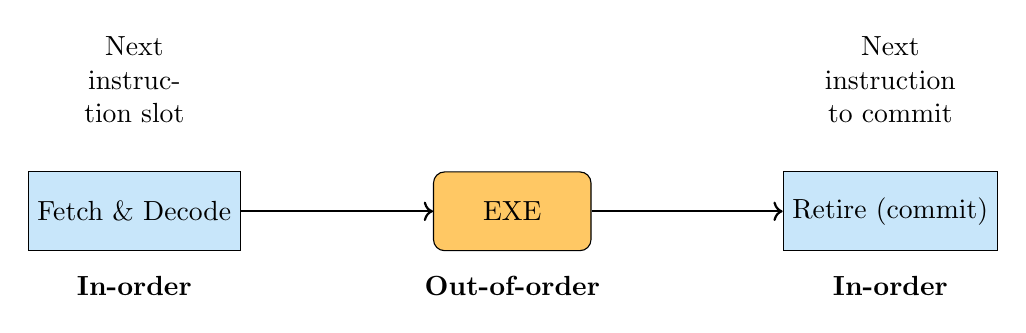
\begin{tikzpicture}[scale=1.2]
        % Stages
        \node[draw, fill=lightblue, minimum width=2cm, minimum height=1cm] (fetch) at (0,0) {Fetch \& Decode};
        \node[draw, fill=highlightorange, minimum width=2cm, minimum height=1cm, rounded corners] (exe) at (4,0) {EXE};
        \node[draw, fill=lightblue, minimum width=2cm, minimum height=1cm] (retire) at (8,0) {Retire (commit)};
        
        % Labels
        \node[below=0.2cm of fetch] {\textbf{In-order}};
        \node[below=0.2cm of exe] {\textbf{Out-of-order}};
        \node[below=0.2cm of retire] {\textbf{In-order}};
        
        % Arrows
        \draw[->, thick] (fetch) -- (exe);
        \draw[->, thick] (exe) -- (retire);
        
        % Annotations
        \node[above=0.5cm of fetch, text width=2cm, align=center] {Next instruction slot};
        \node[above=0.5cm of retire, text width=2cm, align=center] {Next instruction to commit};
    \end{tikzpicture}
    
    \vspace{0.5cm}
    Most modern processors perform fetch/decode and commit stages \textbf{in-order}, while only the execution stage is \textbf{out-of-order}.
\end{frame}

\begin{frame}{ROB (Re-Order Buffer)}
    \begin{itemize}
        \item A common implementation of Register Renaming uses ROB
        \item ROB is a buffer that receives instructions from decode stage in order
        \item The corresponding ROB entry serves as the physical register number for the instruction's destination
        \item After EXE stage, the result is written to the corresponding ROB entry
        \item Instructions commit (exit the processor) in ROB order: an instruction can only commit if the one before it has committed
    \end{itemize}
    
    \vspace{0.5cm}
    \centering
    \drawROB{
        R2/R3 \\
        R4+P0 \\
        R3+R3 \\
        R3+P2 \\
        {} \\
    }
\end{frame}

\begin{frame}{ROB Example - Initial State}
    \begin{columns}
        \column{0.4\textwidth}
        Instructions:
        {\ttfamily\small
        DIV R1, R2, R3\\
        ADD R2, R4, R1\\
        ADD R2, R3, R3\\
        ADD R4, R3, R2
        }
        
        \column{0.6\textwidth}
        \centering
        ROB (Cyclic Buffer):
        
        \drawROB{
            {} \\
            {} \\
            {} \\
            {} \\
            {} \\
        }
        
        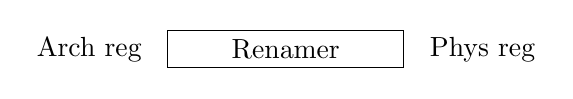
\begin{tikzpicture}
            \node[draw, minimum width=3cm] (renamer) at (0,-2) {Renamer};
            \node[left=0.2cm of renamer] {Arch reg};
            \node[right=0.2cm of renamer] {Phys reg};
        \end{tikzpicture}
    \end{columns}
\end{frame}

\begin{frame}{ROB Example - After First Instruction}
    \begin{columns}
        \column{0.4\textwidth}
        Instructions:
        {\ttfamily\small
        DIV R1, R2, R3  \checkmark\\
        ADD R2, R4, R1\\
        ADD R2, R3, R3\\
        ADD R4, R3, R2
        }
        
        \column{0.6\textwidth}
        \centering
        ROB:
        
        \drawROB{
            R2/R3 \\
            {} \\
            {} \\
            {} \\
            {} \\
        }
        
        \vspace{0.2cm}
        {\small R1 $\rightarrow$ P0}
    \end{columns}
\end{frame}

\begin{frame}{ROB Example - After All Instructions}
    \begin{columns}
        \column{0.4\textwidth}
        Instructions:
        {\ttfamily\small
        DIV R1, R2, R3  \checkmark\\
        ADD R2, R4, R1  \checkmark\\
        ADD R2, R3, R3  \checkmark\\
        ADD R4, R3, R2  \checkmark
        }
        
        \textcolor{correctgreen}{Note: No more False Dependencies! (but RAW still exists)}
        
        \column{0.6\textwidth}
        \centering
        ROB:
        
        \drawROB{
            R2/R3 \\
            R4+P0 \\
            R3+R3 \\
            R3+P2 \\
            {} \\
        }
        
        \vspace{0.2cm}
        {\small 
        R1 $\rightarrow$ P0\\
        R2 $\rightarrow$ P1\\
        R2 $\rightarrow$ P2\\
        R4 $\rightarrow$ P3
        }
    \end{columns}
\end{frame}

\begin{frame}{OOO Scheme Overview}
    \centering
    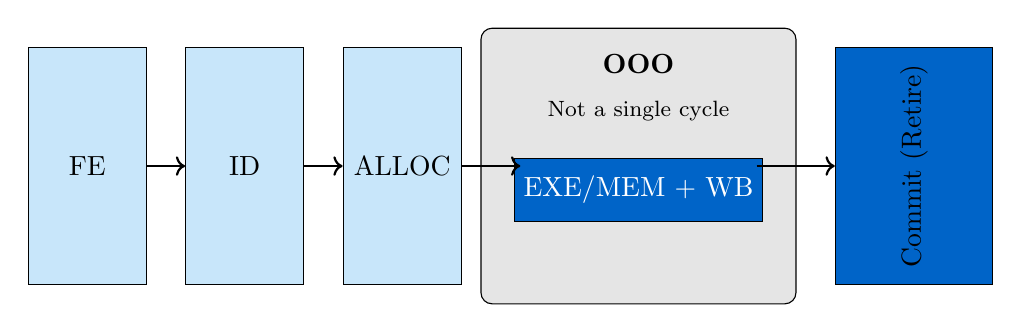
\begin{tikzpicture}[scale=1]
        % Main components
        \node[draw, fill=lightblue, minimum width=1.5cm, minimum height=3cm] (fe) at (0,0) {};
        \node at (0,0) {FE};
        
        \node[draw, fill=lightblue, minimum width=1.5cm, minimum height=3cm] (id) at (2,0) {};
        \node at (2,0) {ID};
        
        \node[draw, fill=lightblue, minimum width=1.5cm, minimum height=3cm] (alloc) at (4,0) {};
        \node at (4,0) {ALLOC};
        
        % OOO section (background box)
        \node[draw, fill=gray!20, rounded corners, minimum width=4cm, minimum height=3.5cm] (ooo) at (7,0) {};
        \node at (7,1.3) {\textbf{OOO}};
        \node at (7,0.7) {\footnotesize Not a single cycle};
        \node[draw, fill=darkblue, text=white, minimum width=3cm, minimum height=0.8cm] at (7,-0.3) {EXE/MEM + WB};
        
        \node[draw, fill=darkblue, text=white, minimum width=2cm, minimum height=3cm] (commit) at (10.5,0) {};
        \node[rotate=90] at (10.5,0) {Commit (Retire)};
        
        % Arrows
        \draw[->, thick] (fe) -- (id);
        \draw[->, thick] (id) -- (alloc);
        \draw[->, thick] (alloc) -- (5.5,0);
        \draw[->, thick] (8.5,0) -- (commit);
    \end{tikzpicture}
\end{frame}

\begin{frame}{Summary}
    \begin{itemize}
        \item \textbf{Problem:} Variable execution times cause pipeline stalls
        \item \textbf{Solution:} Out-of-Order Execution
        \begin{itemize}
            \item Allows independent instructions to execute in parallel
            \item Improves CPI significantly
        \end{itemize}
        \item \textbf{New challenges:} False dependencies (WAR, WAW)
        \item \textbf{Solution:} Register Renaming with ROB
        \begin{itemize}
            \item Maps architectural registers to physical registers
            \item Maintains program correctness while allowing OOO
        \end{itemize}
        \item Modern processors: In-order fetch/commit, Out-of-order execution
    \end{itemize}
\end{frame}

\end{document}